% !TeX document-id = {08592c39-3f56-419f-ac58-b3cbbf9cf119}
% !TeX TXS-program:compile = txs:///xelatex/[--shell-escape]
\documentclass[fontset=windows,openright]{ctexrep}

% =============================================================================
\newcommand{\mytitle}{西北工业大学\\常用数学软件大作业}

% =============================================================================

%
\usepackage{ifxetex}
\usepackage{array}

\renewcommand{\normalsize}{\zihao{5}}
\ctexset{
    chapter = {
        pagestyle=fancy,
        beforeskip=-5pt,
        afterskip=5pt,
        name = {},
        number = \arabic{chapter},
        format = \raggedright \bfseries \Large
    },
    section = {
            format = \raggedright \bfseries 
        }
}

\usepackage{hyperref}
\hypersetup{
    colorlinks=true,
    linkcolor=black,
    citecolor=black,
    filecolor=black,
    urlcolor=black
}
\usepackage[margin=3cm]{geometry}
\usepackage{fancyhdr,lastpage}
\usepackage{fancyqr}
\usepackage{pst-barcode}

% 代码排版
%代码高亮,需要python,pygments支持和 -shell-escape
\usepackage{minted,xcolor}
\definecolor{LightGray}{rgb}{0.92,0.92,0.92}

% Matlab代码排版环境
\newminted[mcode]{matlab}{
	frame=none,
	framesep=2mm,
	baselinestretch=1.2,
	bgcolor=LightGray,
	fontsize=\footnotesize,
	linenos,
	showtabs=false,
	showspaces=false,
	breaklines
}
%% Pyhton 代码排版环境
\newminted[pycode]{python}{
	frame=none,
	framesep=2mm,
	baselinestretch=1.2,
	bgcolor=LightGray,
	fontsize=\footnotesize,
	linenos,
	showtabs=false,
	showspaces=false,
	breaklines
}
\usepackage{amsmath,amssymb}
% \usepackage{fdsymbol}

\pagestyle{fancy}
\renewcommand{\headrulewidth}{1pt} % 设置页眉横线粗细
\renewcommand{\footrulewidth}{1pt} % 设置页脚横线宽度


\usepackage{draftwatermark}
\SetWatermarkText{\hspace*{2cm}DRAFT\hspace*{2cm}DRAFT}  % 水印内容
\SetWatermarkScale{0.5}       % 大小(默认1)
\SetWatermarkLightness{1} % 透明度(0-1,越小越明显)


% \fancyhead[L]{\textsc{\mytitle}}
\fancyhead[C]{{\songti 常用数学软件大作业}}
%\fancyhead[R]{\fancyqr[height=0.8cm, color=black]{20250502v1}\vspace{0.02cm}}
 \fancyhead[R]{}

\fancyhead[L]{}


\fancyfoot[R]{第~\thepage~页,共~\pageref{LastPage}~页}
\fancyfoot[C]{}


% \fancyqrset{gradient=true, l color=blue, r color=teal} % 设置渐变色


%-----------------------------------------------------------------------
\begin{document}

%----------- 封面页
{
    \thispagestyle{empty}
    \vspace*{2cm}
    \begin{center}
        \zihao{1} \heiti \mytitle
    \end{center}

    \vfill

    \heiti \zihao{4}

    \begin{center}
        \renewcommand{\arraystretch}{2} % Adjust row height
        \begin{tabular}{cw{c}{5cm}}           
            学期: & { 2024-2025学年春季学期}  \\ \cline{2-2}
            学号: & {\ziju{0.5}  202xxxxxxx}  \\ \cline{2-2}
            姓名: & {\ziju{0.5}  张三}  \\ \cline{2-2}
        \end{tabular}
    \end{center}
    \vspace{3cm}
    \begin{center}
        西北工业大学 \\
        2025年6月20日
    \end{center}
}
\newpage   


\newpage % 加入空白页
\cleardoublepage

%----------- 目录部分
%{
%    % \pagestyle{empty}
%    \fancyhf{}
%    \tableofcontents \vfill
%    \newpage 
%    \cleardoublepage
    \setcounter{page}{1}
%}
% 示例内容

%---------- 正文内容
\chapter{第一部分} \label{section:introduction}
\section{油料储量问题}

\subsection{问题描述}
储油罐由中间圆柱形和两端半球形组成,圆柱长度$L=6\text{m}$,球体半径$R=1.5\text{m}$。油罐可能水平放置或与水平面有$5^\circ$、$8^\circ$的倾角。$H$为O点距油罐中油料平面的距离,在$0$到$2\text{m}$区间变化。

\subsection{数学模型}
油料体积$V$由圆柱部分和两个半球部分的体积组成:

水平放置时($\theta=0^\circ$):
\begin{itemize}
    \item 当$0 \leq H \leq R$时:$V = \pi H^2 \left(R - \frac{H}{3}\right)$
    \item 当$R < H < 2R$时:$V = \frac{2}{3}\pi R^3 + \pi R^2(H-R)$
    \item 当$H \geq 2R$时:$V = \frac{2}{3}\pi R^3 + \pi R^2 L$
\end{itemize}

倾斜放置时($\theta > 0^\circ$),需要通过数值积分计算油料体积。

\subsection{计算结果}
\begin{figure}[h]
    \centering
    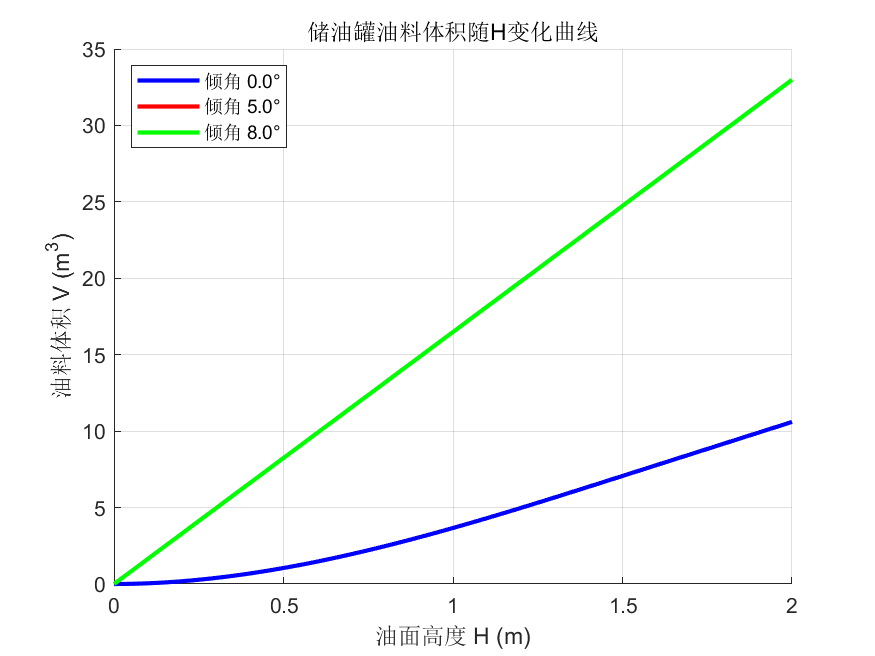
\includegraphics[width=0.8\textwidth]{oil_volume.png}
    \caption{储油罐油料体积随H变化曲线}
    \label{fig:oil_volume}
\end{figure}

从图\ref{fig:oil_volume}可以看出,随着倾角的增大,相同油面高度$H$对应的油料体积减小。

\chapter{第二部分}
\section{土方量计算问题}

\subsection{问题描述}
根据给定的地形坐标数据(coords.csv),计算将该区域平整后再向下开挖2.5m的土方量。采用Delaunay三角剖分构建地形表面,然后按照三棱柱方法计算体积。

\subsection{计算方法}
\begin{enumerate}
    \item 读取坐标和高程数据
    \item 生成Delaunay三角网格
    \item 计算平整基准面高程(取所有点高程平均值)
    \item 对每个三角形:
    \begin{itemize}
        \item 计算三角形面积
        \item 计算平均高程与基准面的高差
        \item 计算三棱柱体积
    \end{itemize}
    \item 累加所有三棱柱体积得到总土方量
\end{enumerate}

\subsection{计算结果}
\begin{figure}[h]
    \centering
    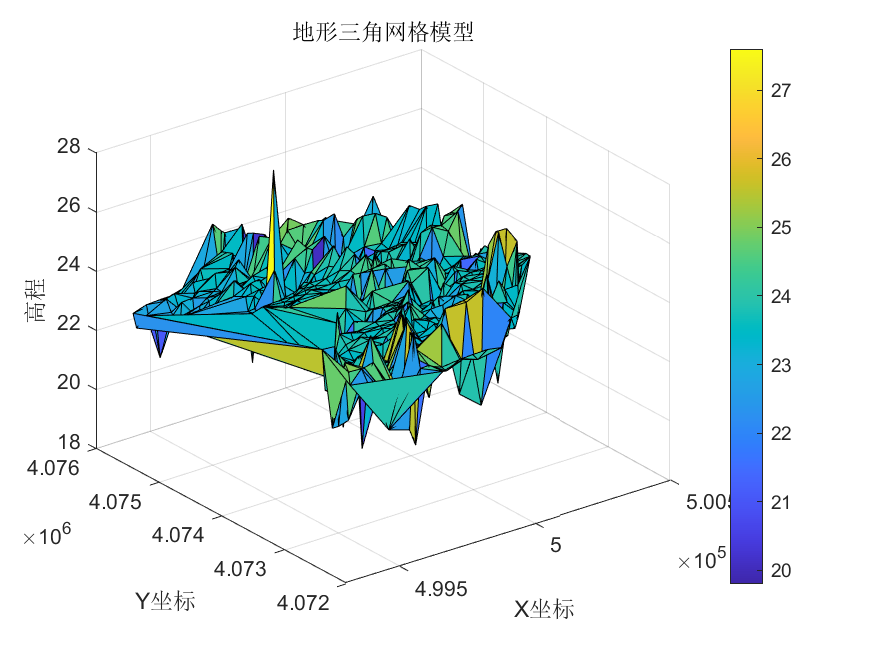
\includegraphics[width=0.8\textwidth]{terrain_model.png}
    \caption{地形三角网格模型}
    \label{fig:terrain}
\end{figure}

计算得到:
\begin{itemize}
    \item 平整土方量:\textbf{153375.11 m³}
    \item 开挖2.5m土方量:\textbf{8384526.94 m³}
\end{itemize}

\chapter{第三部分}
\section{一维下料问题}

\subsection{问题描述}
从长度为$L$的标准件中切割出不同长度的坯料,要求满足各种坯料的需求数量,且使用的标准件数量最少。

\subsection{数学模型}
设:
\begin{itemize}
    \item 标准件长度:$L$
    \item 坯料种类:$m$,长度分别为$l_1, l_2, \ldots, l_m$
    \item 坯料需求数量:$b_1, b_2, \ldots, b_m$
    \item 切割方式:$k$种,第$i$种方式重复$x_i$次
    \item 第$i$种切割方式得到第$j$种坯料数量:$c_{ij}$
\end{itemize}

目标函数:
\[ \text{最小化} \sum_{i=1}^k x_i \]

约束条件:
\[ \sum_{i=1}^k c_{ij} x_i \geq b_j, \quad j=1,\ldots,m \]
\[ \sum_{j=1}^m c_{ij} l_j \leq L, \quad i=1,\ldots,k \]
\[ x_i \geq 0 \text{且为整数} \]

材料利用率:
\[ \eta = \frac{\sum_{j=1}^m b_j l_j}{L \sum_{i=1}^k x_i} \times 100\% \]

\subsection{计算结果}
以第一组数据为例:
\begin{itemize}
    \item 标准件长度:$L=100$
    \item 坯料长度及需求:
    \begin{tabular}{|c|c|c|c|c|c|}
        \hline
        坯料长度(m) & 46.3 & 40.5 & 32.4 & 25.6 & 18.2 \\
        \hline
        需求数量 & 100 & 200 & 200 & 200 & 200 \\
        \hline
    \end{tabular}
\end{itemize}

MATLAB计算得到:
\begin{itemize}
    \item 最少需要标准件数量:\textbf{2.860000e+02}
    \item 材料利用率:\textbf{97.80\%}
    \item 最优切割方案:
    \begin{mcode}
    方式10 (使用2.100000e+01次): 1根25.6m 4根18.2m 
    方式31 (使用2次): 1根40.5m 3根18.2m 
    方式34 (使用2.000000e+00次): 1根40.5m 2根25.6m 
    方式37 (使用1.250000e+02次): 1根40.5m 1根32.4m 1根25.6m 
    方式39 (使用36次): 2根40.5m 1根18.2m 
    方式45 (使用2.500000e+01次): 1根46.3m 2根25.6m 
    方式47 (使用7.500000e+01次): 1根46.3m 1根32.4m 1根18.2m 
    \end{mcode}
\end{itemize}

\end{document}